\section{Results}
\label{sec:results}
This section introduces the estimation results from the baseline model, in which the central part is the forecast error variance decomposition (FEVD). I begin with a moments comparison between the estimated model and the data.

\subsection{Moments}
\label{sec:results:moments}
Table~\ref{tab:varcmp:gov-data} shows the comparison of mean and variance implied by the model and the data. Though most of the moments are close, the variance of the hours worked is extremely high compared with the data. To investigate this result, we can look into the log-linearized equations to write the labor input by state variables out of the labor market.
\begin{equation}\label{eq:n-decomp}
    \hat N_t = \frac{\hat{mc}_t + \alpha \hat{k}^s_t + \hat{\mu}_{a,t} - \theta_w \sigma \hat{c}_t}{\alpha + \theta_w \psi}
\end{equation}

% Auto-generated by test_variance_decomp_nocap.m
% file_name: gov_data

\begin{table}[!htbp]
\centering
\caption{Model-implied and data moments (mean and variance) for the baseline observables (output, inflation, interest rate, hours, investment, and government spending).}
\label{tab:varcmp:gov-data}
\begin{tabular}{l r @{\hspace{2em}} r c r @{\hspace{2em}} r}
\hline\hline
 & \multicolumn{2}{c}{Mean} & & \multicolumn{2}{c}{Variance} \\ 
\cline{2-3}\cline{5-6}
Observable & Model & Data & & Model & Data \\ 
\hline
Output & 0.33 & 0.56 & & 0.67 & 0.34 \\ 
Inflation & 4.05 & 3.08 & & 5.09 & 2.16 \\ 
Interest rate & 7.15 & 6.05 & & 8.33 & 5.01 \\ 
Hours & 0.96 & 0.00 & & 31.86 & 6.37 \\ 
Investment & 0.33 & 0.57 & & 3.87 & 2.53 \\ 
Gov. spending & 0.33 & 0.31 & & 0.82 & 0.85 \\ 
\hline
\end{tabular}
\end{table}


I decompose the stationary variance of $\hat N_t$ into the four parts laying on the numerator. Specifically, the stationary variance is computed by
$$ \mathrm{Var}(\bar s) = \mathrm{Var}(\Phi \bar s + R \varepsilon) = \Phi \mathrm{Var}(\bar s) \Phi' + R \mathrm{Var}(\varepsilon) R',$$
and then $R^2$ is computed according to equation \eqref{eq:n-decomp} and the variance of each state variables. The result is summarized in Table~\ref{tab:hours-R2:gov-data}. 

% Auto-generated by test_hours_R2.m
% file_name: gov_data

\begin{table}[!htbp]
\centering
\caption{Decomposing model-implied hours volatility. $R^2=\mathrm{corr}(N_t,x_t)^2$ from regressing model-implied hours on each component $x_t$, i.e.\ the share of $\mathrm{Var}(N_t)$ linearly accounted for by co-movement with that component. Moments are theoretical (unconditional) second moments, $\Sigma=\Phi\Sigma\Phi'+R\,Se\,R'$.}
\label{tab:hours-R2:gov-data}
\begin{tabular}{l r r}
\hline\hline
Component & $\mathrm{corr}(N_t,x_t)$ & $R^2$ (\%) \\ 
\hline
Consumption, $\hat{c}_t$ & +0.907 & 82.29 \\
Marginal cost, $\hat{mc}_t$ & +0.061 & 0.37 \\ 
Capital services, $\hat{k}_t^s$ & -0.030 & 0.09 \\ 
Technology, $\hat{\mu}_{a, t}$ & +0.087 & 0.76 \\ 
\hline
\end{tabular}
\end{table}


In such decomposition, the high volatility of hours worked mainly comes from the volatile consumption log-deviation (level) $\hat c_t$. Though in the data, the variance of $\hat c_t$ is just about $2.8$, the model implied counterpart is $39.23$ as shown in Table~\ref{tab:var_level_sw2007_vs_baseline}. While it is normal to think that consumption is volatile in the baseline estimation, because the consumption data is not used in the data set, Table~\ref{tab:var_level_sw2007_vs_baseline} also shows that this problem persists in the workhorse model in \cite{smetsShocksFrictionsUS2007}. I compute this statistic from the replication package of \cite{smetsShocksFrictionsUS2007} directly, the value reaches to $33.75$ as well.

% Unconditional (theoretical) variance of the LEVEL of consumption and hours
% SW2007 moments computed in Dynare at the SW posterior mode; baseline_model
% moments at its estimated posterior; data = sample variance of the detrended
% log series actually used in estimation.
\begin{table}[htbp]
\centering
\caption{Model-implied vs.\ data variance of the \emph{level} of consumption and
hours worked. Data variance of consumption level is computed by the cyclical term detrended by OLS constant and time-liear term. The \cite{smetsShocksFrictionsUS2007} column reports the theoretical unconditional moments of the original Smets--Wouters (2007) model. If we assume state variables follow AR(1) processes, the gap between the model levels and the data is driven by persistence:
$\mathrm{Var}(\text{level})= \mathrm{Var}(\text{growth})/[2(1-\rho_1)]$.}
\label{tab:var_level_sw2007_vs_baseline}
\begin{tabular}{lccc}
\hline\hline
Variable & \cite{smetsShocksFrictionsUS2007} & Baseline model & Data \\
\hline
Consumption ($c$) & 33.75 & 39.23 & 2.80 \\
\quad $\rho_1$    & 0.993 & 0.996 & 0.901 \\
Hours worked ($N$)& 8.85  & 32.22 & 6.29 \\
\quad $\rho_1$    & 0.975 & 0.993 & 0.907 \\
\hline\hline
\end{tabular}
\end{table}


However, the variance of labor input differs quite a lot. This is because \cite{smetsShocksFrictionsUS2007} adds a wage markup shock $\mu_{w,t}$ between the marginal rate of substitution and the real wage
$$\hat{\pi}_t^w = \beta \mathbb{E}_t \hat{\pi}_{t+1}^w - \kappa_w \underbrace{\left(\hat{w}_t - \hat{mrs}_t+ \frac{1}{\kappa_w}\mu_{w, t}\right) }_{\text{wage markup}} .$$

By adding such shock, wage is less tied with $MRS_t$, and thus it has more freedom to fit with the data. In Section~\ref{sec:robustness:sw}, the estimation based on the \cite{smetsShocksFrictionsUS2007} model shows a much better fit for the variance of hours worked, and the FEVD analysis in Table~\ref{tab:vd:sw-type-no-rel} also shows the strong influence of the wage markup shock on hours worked and wage growth.

Nevertheless, from the wage Phillips curve equation, it is natural to think that $\kappa_w$ will play an important role on the connection between consumption and labor input. Actually, by computing $\kappa_w$ under posterior in Section~\ref{sec:robustness:sw}, it is only tiny $0.006$. But if we drop the wage markup shock, the weak link between $MRS_t$ and wage effectively let the wage to be nearly static, and it is why even if the parameter $\theta_w$ exists in the simplified wage setting equation, its posterior still stays about $0.5$.

\subsection{Forecast Error Variance Decomposition}
\label{sec:results:fevd}
Table~\ref{tab:vd:gov-data} is the unconditional FEVD computed by a 400-iteration algorithm because directly solving the Lyapunov equation is not numerically stable in this model. As illustrated in the table, both IST shock and investment demand shock have important effects on the business cycle. The sum of these two shocks can account for about 65\% of the forecast error of the output, 45\% of inflation, and 90\% of hours worked. This result is similar to \cite{justinianoInvestmentShocksBusiness2010}, who claimed that the IST shock contributes about 50\% of the forecast error of the output and 60\% of hours worked.

Separately, investment demand shock alone contributes about 40\% of the forecast error of the output, and about 50\% of the investment. However, investment demand shock contributes much less for the hours worked than IST shock. 

% Auto-generated by test_variance_decomp_nocap.m
% file_name: gov_data

\begin{table}[!htbp]
\centering
\caption{Unconditional FEVD (\%) for the baseline estimation, by government spending ($\varepsilon_g$), IST ($\varepsilon_s$), monetary policy ($\varepsilon_R$), technology ($\varepsilon_a$), and investment demand ($\varepsilon_d$) shocks.}
\label{tab:vd:gov-data}
\begin{tabular}{l @{\hspace{2em}} r @{\hspace{2em}} r @{\hspace{2em}} r @{\hspace{2em}} r @{\hspace{2em}} r}
\hline\hline
Observable & $\varepsilon_g$ & $\varepsilon_s$ & $\varepsilon_R$ & $\varepsilon_a$ & $\varepsilon_d$ \\ 
\hline
Output & 4.63 & 15.55 & 11.00 & 27.12 & 41.69 \\ 
Inflation & 0.32 & 39.26 & 12.87 & 40.14 & 7.41 \\ 
Interest rate & 0.37 & 55.06 & 5.48 & 31.22 & 7.87 \\ 
Hours & 4.34 & 90.19 & 0.08 & 3.56 & 1.83 \\ 
Investment & 0.11 & 36.23 & 0.15 & 12.04 & 51.48 \\ 
Gov. spending & 99.87 & 0.02 & 0.01 & 0.04 & 0.06 \\ 
\hline
\end{tabular}
\end{table}


The first reason is the high autocorrelation of IST shock. As shown in Table~\ref{tab:prior_posterior_params}, $\rho_s$ is quite close to the unit root, while $\rho_d = 0.87$ in the posterior. Second, IST shock triggers a hump-shape adjustment of investment due to the investment adjustment cost. Therefore, its peak arrives late and thus more persistent. By contrast, investment demand shock doesn't have such effect, because it changes the investment exogenously. Finally, the substitution effect of IST shock is strong. As shown in Figure~\ref{fig:compare_irf}, IST shock causes the instant negative wage response but the positive labor input response. The story behind it is that the shock moves the labor supply curve toward the right, reflecting the incentive to save more today because of the cheap investment. The negative response of consumption and the nearly static output confirm the intertemporal substitution effect, as they purely increase saving and decrease consumption. On the other side, the investment demand shock shows less substitution effect. As the wage and labor input increase simultaneously, it is the movement of the labor demand curve that dominates the labor market. Though consumption decreases as well, output increases a lot, which shows that households haven't shifted consumption to investment completely. This is the wealth effect discussed in \cite{nireiOriginsPropagationAnimal} and \cite{greenwoodInvestmentCapacityUtilization1988}: higher investment means higher output in the future, and thus higher lifetime wealth.

\begin{figure}
    \centering
    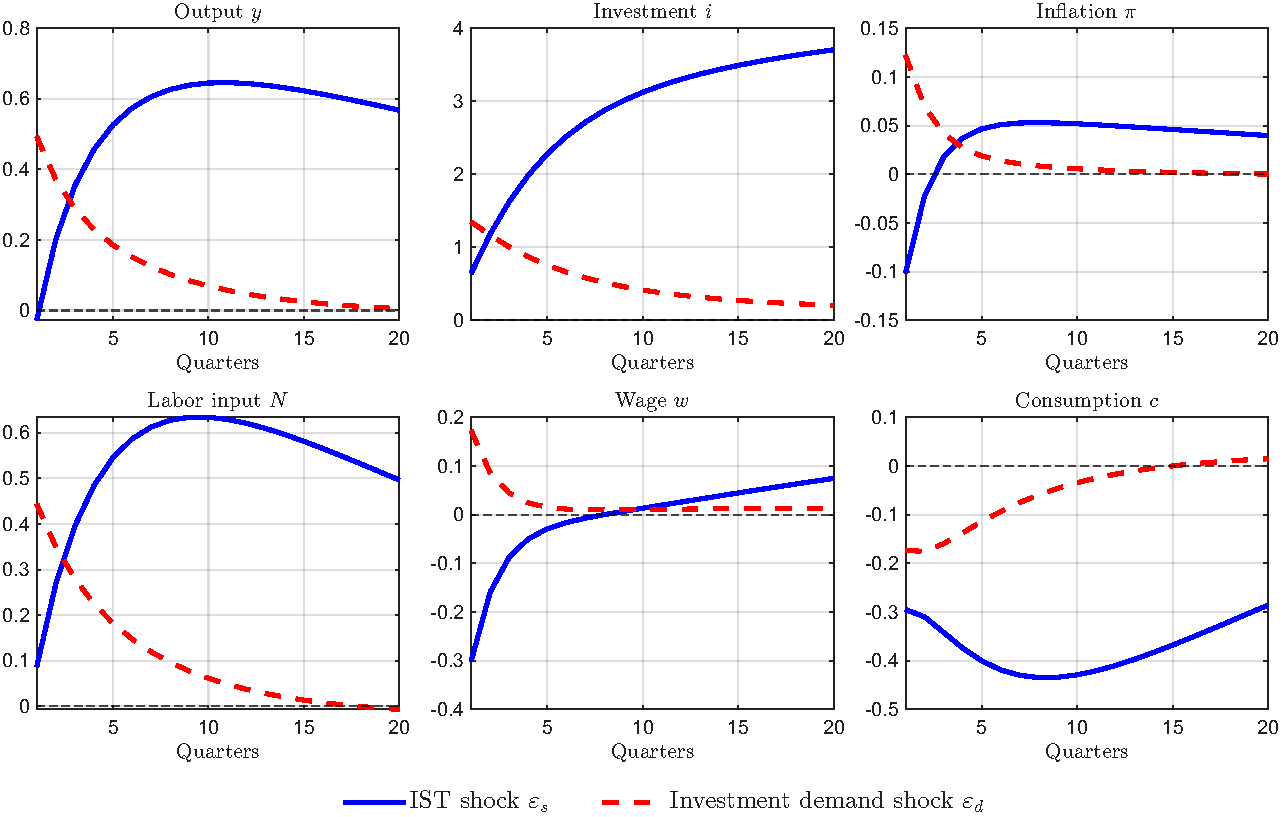
\includegraphics[width=0.9\textwidth]{figures/compare_irf_gov_data.pdf}
    \caption{Impulse responses of output, investment, inflation, labor input, wage, and consumption to one-standard-deviation IST and investment demand shocks (baseline estimation; horizon: 20 quarters).}
    \label{fig:compare_irf}
\end{figure}

Nevertheless, \cite{justinianoInvestmentShocksBusiness2010} uses the frequency based FEVD. To faciliate comparing, Table~\ref{tab:fevd-frequency:gov-data} shows the FEVD result based on the same methodology.

% Auto-generated by test_fevd_frequency.m
% file_name: gov_data
% band: 6--32 quarters; nbins=500

\begin{table}[!htbp]
\centering
\caption{Frequency-domain FEVD (\%) for the business-cycle band (6--32 quarters), with measurement error included (baseline estimation; 500 frequency bins).}
\label{tab:fevd-frequency:gov-data}
\begin{tabular}{l @{\hspace{2em}}r @{\hspace{2em}}r @{\hspace{2em}}r @{\hspace{2em}}r @{\hspace{2em}}r @{\hspace{2em}}r}
\hline\hline
Observable & $\varepsilon_g$ & $\varepsilon_{s}$ & $\varepsilon_R$ & $\varepsilon_a$ & $\varepsilon_{d}$ & $\mathrm{meas}$ \\ 
\hline
Output & 1.44 & 28.15 & 2.16 & 57.59 & 9.77 & 0.89 \\ 
Inflation & 0.13 & 16.26 & 17.73 & 59.52 & 5.06 & 1.29 \\ 
Interest rate & 0.16 & 22.76 & 9.76 & 58.55 & 6.33 & 2.45 \\ 
Hours & 2.68 & 49.48 & 1.49 & 23.25 & 16.69 & 6.42 \\ 
Investment & 0.19 & 54.18 & 0.18 & 28.69 & 15.72 & 1.03 \\ 
Gov. spending & 95.93 & 0.02 & 0.00 & 0.04 & 0.01 & 4.00 \\ 
\hline
\end{tabular}
\end{table}


The result shows that the aggregate technology has a much stronger effect on the business cycle, which accounts for about $50\%$ for output, inflation and nominal interest rate. IST shock contributes for $28.15\%$ of output, $16.26\%$ of inflation, $54.14\%$ of investment, and $49.48\%$ of hours worked. Meanwhile, investment demand shock is less important, accounting for $9.77\%$ of output, $5.06\%$ of inflation, $15.72\%$ of investment and $16.69\%$ of hours worked. 

Compared with the unconditional FEVD analysis in Table~\ref{tab:varcmp:gov-data}, the frequency FEVD restricts the impact to between 6 and 32 quarters. From the IRF plot in Figure~\ref{fig:compare_irf}, we can observe that the effect caused by investment demand shock almost converges to zero after 6 periods, which explains why it contributes less in frequency FEVD result.

\subsection{Inflation Impact}
\label{sec:results:inf}
Another interesting point in Figure~\ref{fig:compare_irf} is that the IST shock results in deflation in the first periods, while the investment demand shock generates inflation. Although this difference is documented in \cite{nireiOriginsPropagationAnimal}, which can be explained by the competition between substitution effect and wealth effect introduced before, \cite{justinianoInvestmentShocksBusiness2010} and Section \ref{sec:robustness} in this paper propose the contrary result---IST shock raises deflationary effect. Comparing the posterior, $\rho_{s}$ and $\psi_u$ show a big difference. Figure~\ref{fig:irf_rho_ist_psi_u_sign_flip} tests the inflation response to IST shock under various values of $\rho_{s}$ and $\psi_u$, where $\psi_u$ is defined from the household first-order condition of capital utilization rate \eqref{eq:util_foc},
$$\hat r^k_t = \frac{a''(1)}{a'(1)}\,\hat u_t \equiv \frac{\psi_u}{1 - \psi_u}\,\hat u_t.$$

\begin{figure}
    \centering
    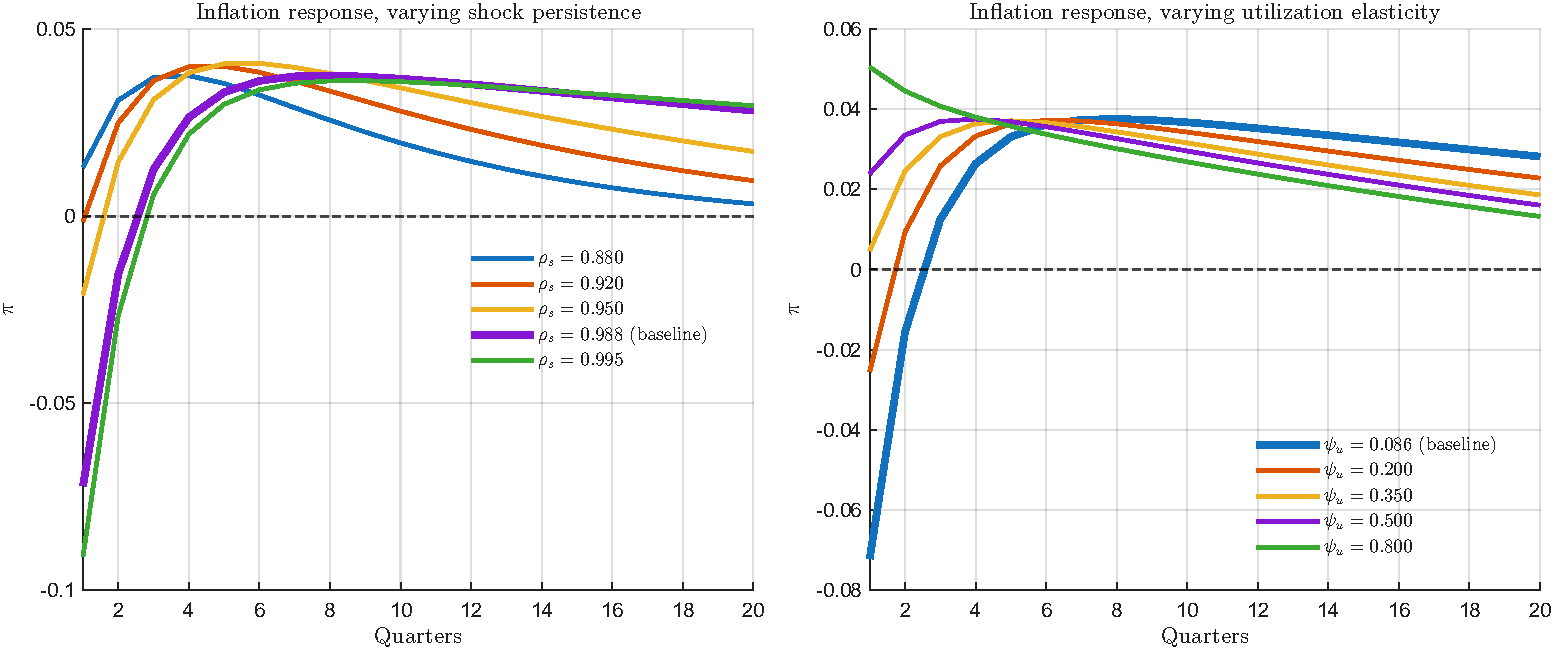
\includegraphics[width=0.7\textwidth]{figures/irf_rho_ist_psi_u_sign_flip.pdf}
    \caption{The sign of the inflation response to an IST shock depends on the estimated shock persistence $\rho_{s}$ and the capital-utilization elasticity $\psi_u$.}
    \label{fig:irf_rho_ist_psi_u_sign_flip}
\end{figure}

Under high $\rho_s$ and low $\psi_u$, the deflationary result is produced. However, inflationary result can be shown if $\rho_s$ is below $0.92$ or $\psi_u$ is above $0.32$,  keeping all other parameters unchanged. To understand the result, we can write the inflation as the summation of present discounted value of marginal cost,
\begin{equation}\label{eq:inf-mc}
    \hat{\pi}_t = \beta \mathbb{E}_t \hat{\pi}_{t+1} + \kappa_p \widehat{mc}_t \implies \hat{\pi}_t = \kappa_p \underbrace{\sum_{j = 0}^\infty \beta^j \mathbb{E}_t[\widehat{mc}_{t+j}]}_{= \, \text{PDV}(mc)}.
\end{equation}

Furthermore, there are two channel to influence the marginal cost---wage and capital rental rate, shown in Figure~\ref{fig:mc_decomposition_rk_psi_u}. The first shows that under low $\psi_u$, marginal cost is mainly accounted by the wage channel, while capital rental rate has only small effect in the first few periods. To understand this, we associate capital rental rate with firm's cost minimization decision \eqref{eq:loglin_factorprices} and households' capital utilization decision \eqref{eq:loglin_u},
\begin{equation}\label{eq:mpk-equal-rk}
    \begin{cases}
        \hat r^k_t = \hat w_t + \hat N_t - \hat K_{t-1} - \hat u_t\\
        \hat r^k_t = \frac{\psi_u}{1 - \psi_u}\,\hat u_t
    \end{cases}
    \implies
    \hat r^k_t = \psi_u \left(\hat w_t + \hat N_t - \hat k_{t-1}\right).
\end{equation}

\begin{figure}
    \centering
    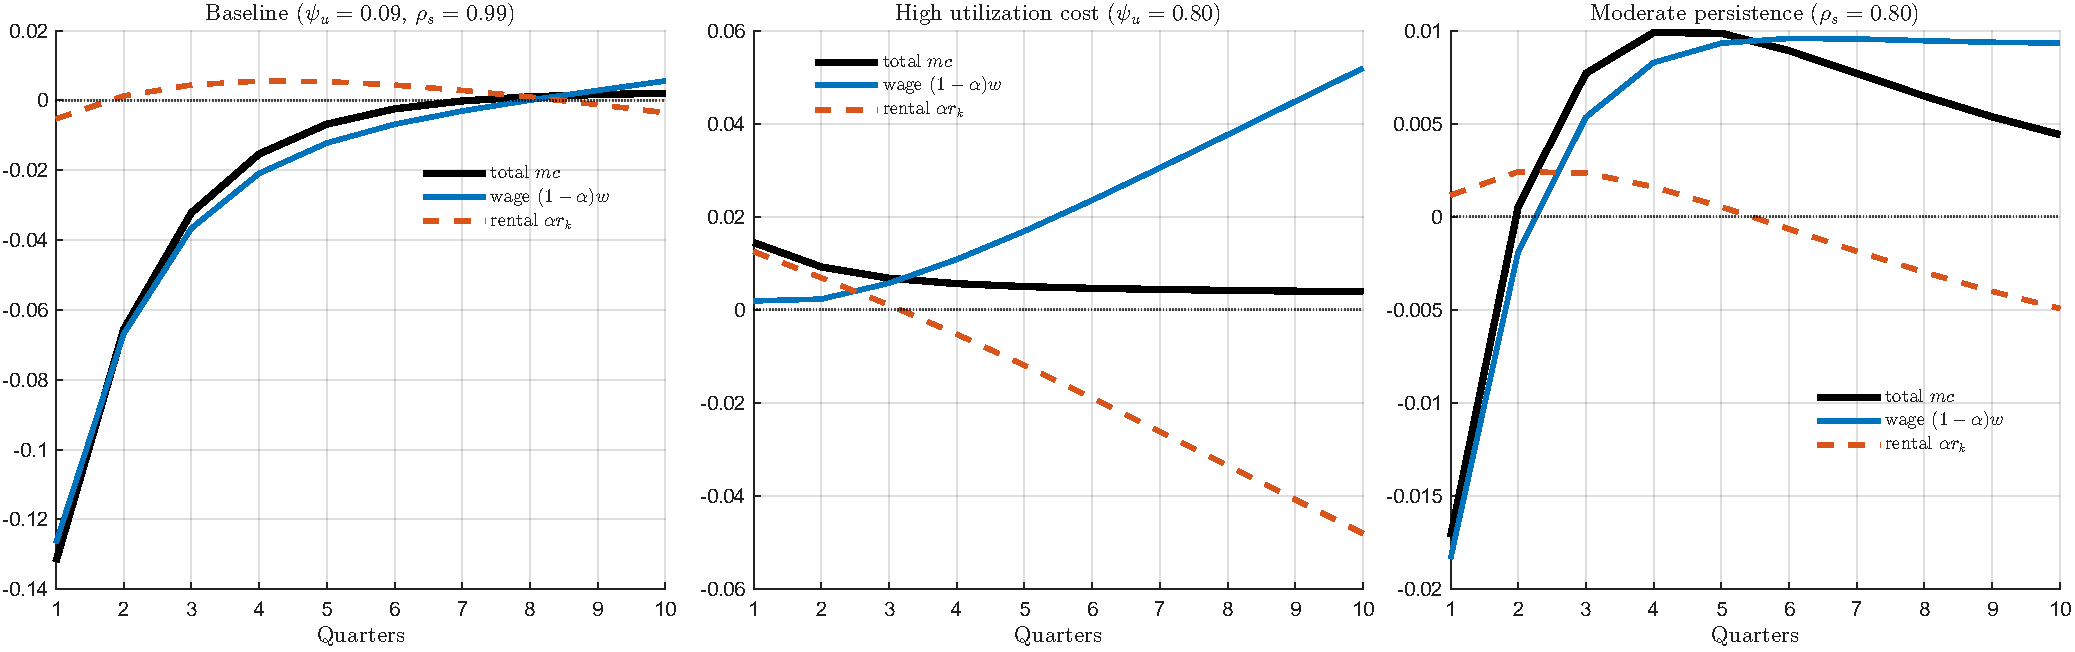
\includegraphics[width=0.9\textwidth]{figures/mc_decomposition_rk_psi_u.pdf}
    \caption{Decomposing the marginal-cost response to an IST shock: a wage channel against a capital-rental channel.}
    \label{fig:mc_decomposition_rk_psi_u}
\end{figure}

Equation \eqref{eq:mpk-equal-rk} shows $\hat r^k_t$ will only move $\psi_u$ fraction of $\hat w_t + \hat N_t$, as $\hat k_{t-1}$ is predetermined. First, under baseline result, $\hat w_t$ and $\hat N_t$ move to the opposite direction, which cancels out the absolute value of the difference. Second, the posterior of $\psi_u$ is only about $0.1$, dampening the magnitude a lot. However, the second panel of Figure~\ref{fig:mc_decomposition_rk_psi_u} shows the capital rental rate channel becomes important as $\psi_u$ becomes large, leading to the inflationary result. To understand this change, we can recall the definition of $\psi_u$ again. As $\frac{a''(1)}{a'(1)} = \frac{\psi_u}{1 - \psi_u}$, increase of $\psi_u$ implies $a''(1)$ becomes relatively larger. This means the adjustment cost function is steeper around the steady state. When the IST shock creates the increasing labor supply, marginal productivity of capital increases and thus capital demand increases. However, capital supply can hardly adjust due to the expensive adjustment cost. Therefore, the strong movement of the capital demand curve results in the high rental rate in the first few periods.

Understanding the role of $\psi_u$ helps the further analysis about $\rho_s$. Since $\psi_u$ is small in baseline posterior, we can focus on the wage channel. When $\rho_s$ decreases, the IST shock will persists shorter period once it arrives. Suppose IST shock is positive, then household will save more for shorter period when the investment is cheap, and thus wage will decrease for shorter time. As the current inflation is the summation of future marginal cost shown in equation~\eqref{eq:inf-mc}, it will be positive once the summation of negative initial terms is outweighed by the positive tail, as shown in the third panel of Figure~\ref{fig:mc_decomposition_rk_psi_u}.

It is worth stressing that the inflation impact under the IST shock is also sensitive to many other parameter values, such as the wage sticky parameter and the Phillips curve parameter, shown in Figure~\ref{fig:ist_sign_robustness}. Although the sign of the inflation impact is not robust to the parameter value choice, the sign of the wage impact shows a stable result in this exercise. However, I acknowledge the limitation of such an exercise: it alters parameters one by one, but cannot investigate the effect of simultaneous movement among several parameters. In fact, \cite{justinianoInvestmentShocksBusiness2010} shows the positive wage impact under IST shock.

\begin{figure}
    \centering
    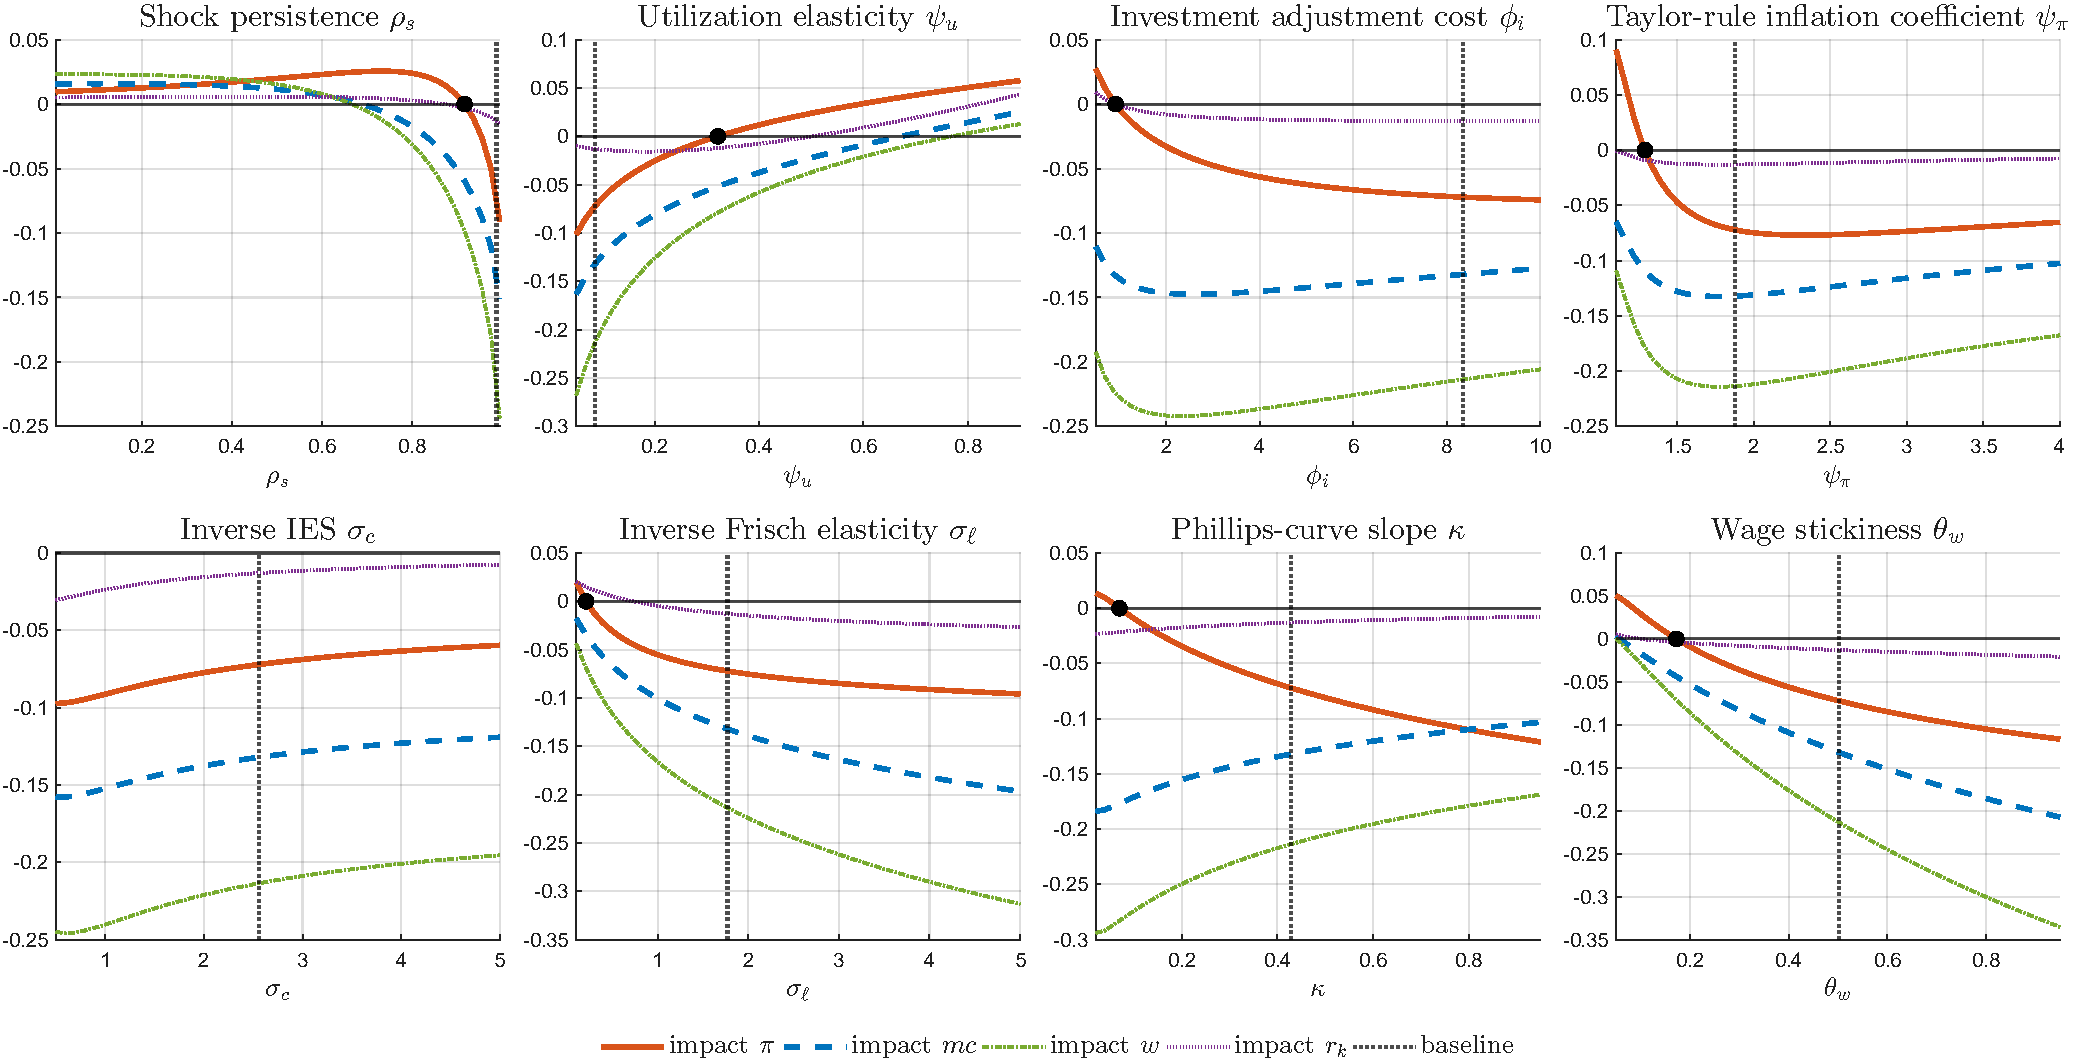
\includegraphics[width=\textwidth]{figures/ist_sign_robustness.pdf}
    \caption{Sensitivity of the sign of the impact inflation response to an IST shock. Each panel varies one parameter over a wide grid}
    \label{fig:ist_sign_robustness}
\end{figure}

On the other side, Figure~\ref{fig:inv_demand_mc_decomposition} shows the evidence about the robust inflationary effect of investment demand shock. The left panel shows both wage and capital rental rate increase under investment shock. This is because the shift of labor demand curve pushes up both labor input and wage, and thus capital rental rate increases by equation~\eqref{eq:mpk-equal-rk}. The right panel shows that the inflation impact is positive under the investment demand shock across all 500 selected draws. Moreover, as shown in Figure~\ref{fig:inv_demand_sign_robustnes}, the parameter sweep exercise confirms the robustness of this effect, and the wage impact remains positive during every single parameter sweep.

\begin{figure}
    \centering
    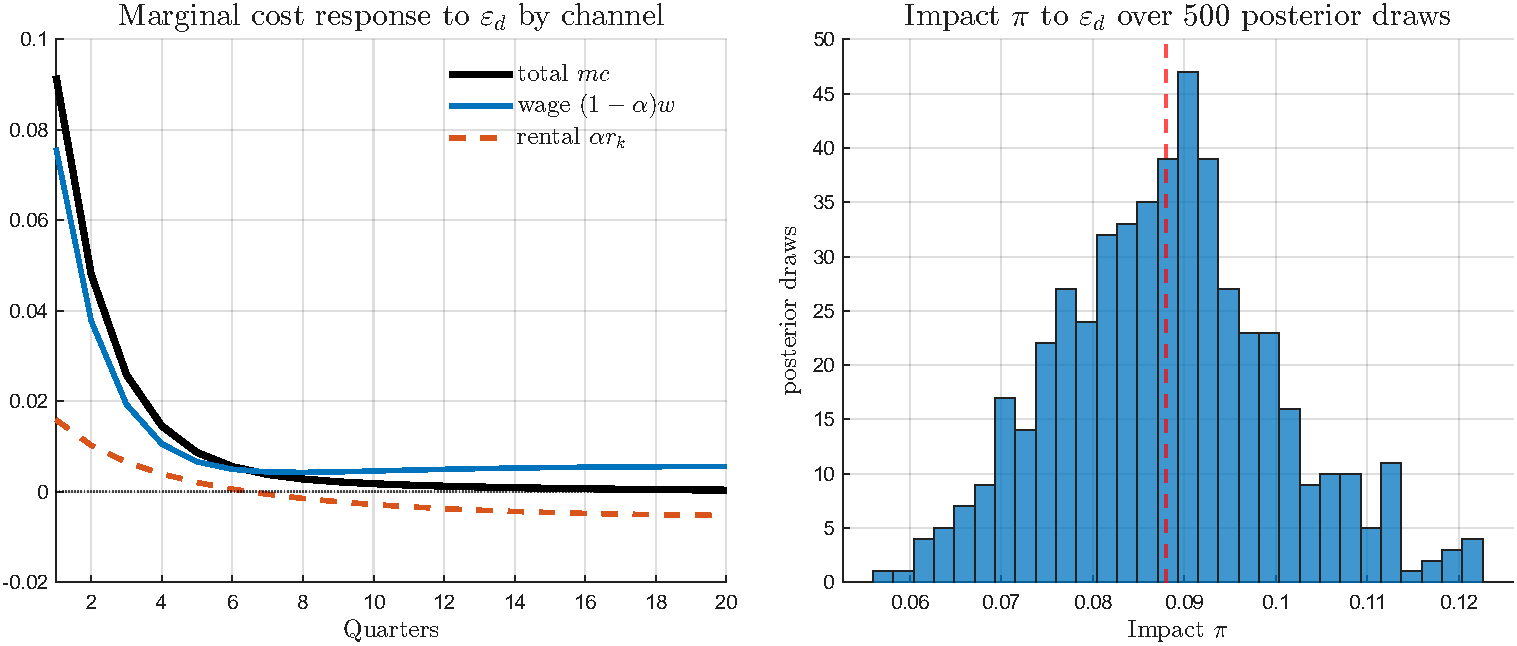
\includegraphics[width=0.7\textwidth]{figures/inv_demand_mc_decomposition.pdf}
    \caption{Robustness of the inflationary response to an investment-demand shock. \textit{Left panel.} Channel decomposition of the real marginal-cost response to a unit investment-demand shock at the baseline posterior mean. \textit{Right panel.} Impact inflation \(\hat\pi_1\) in response to a unit investment-demand shock across 500 posterior MH draws that are selected linarly across index among MH samples after burn-in.}
    \label{fig:inv_demand_mc_decomposition}
\end{figure}

\begin{figure}
    \centering
    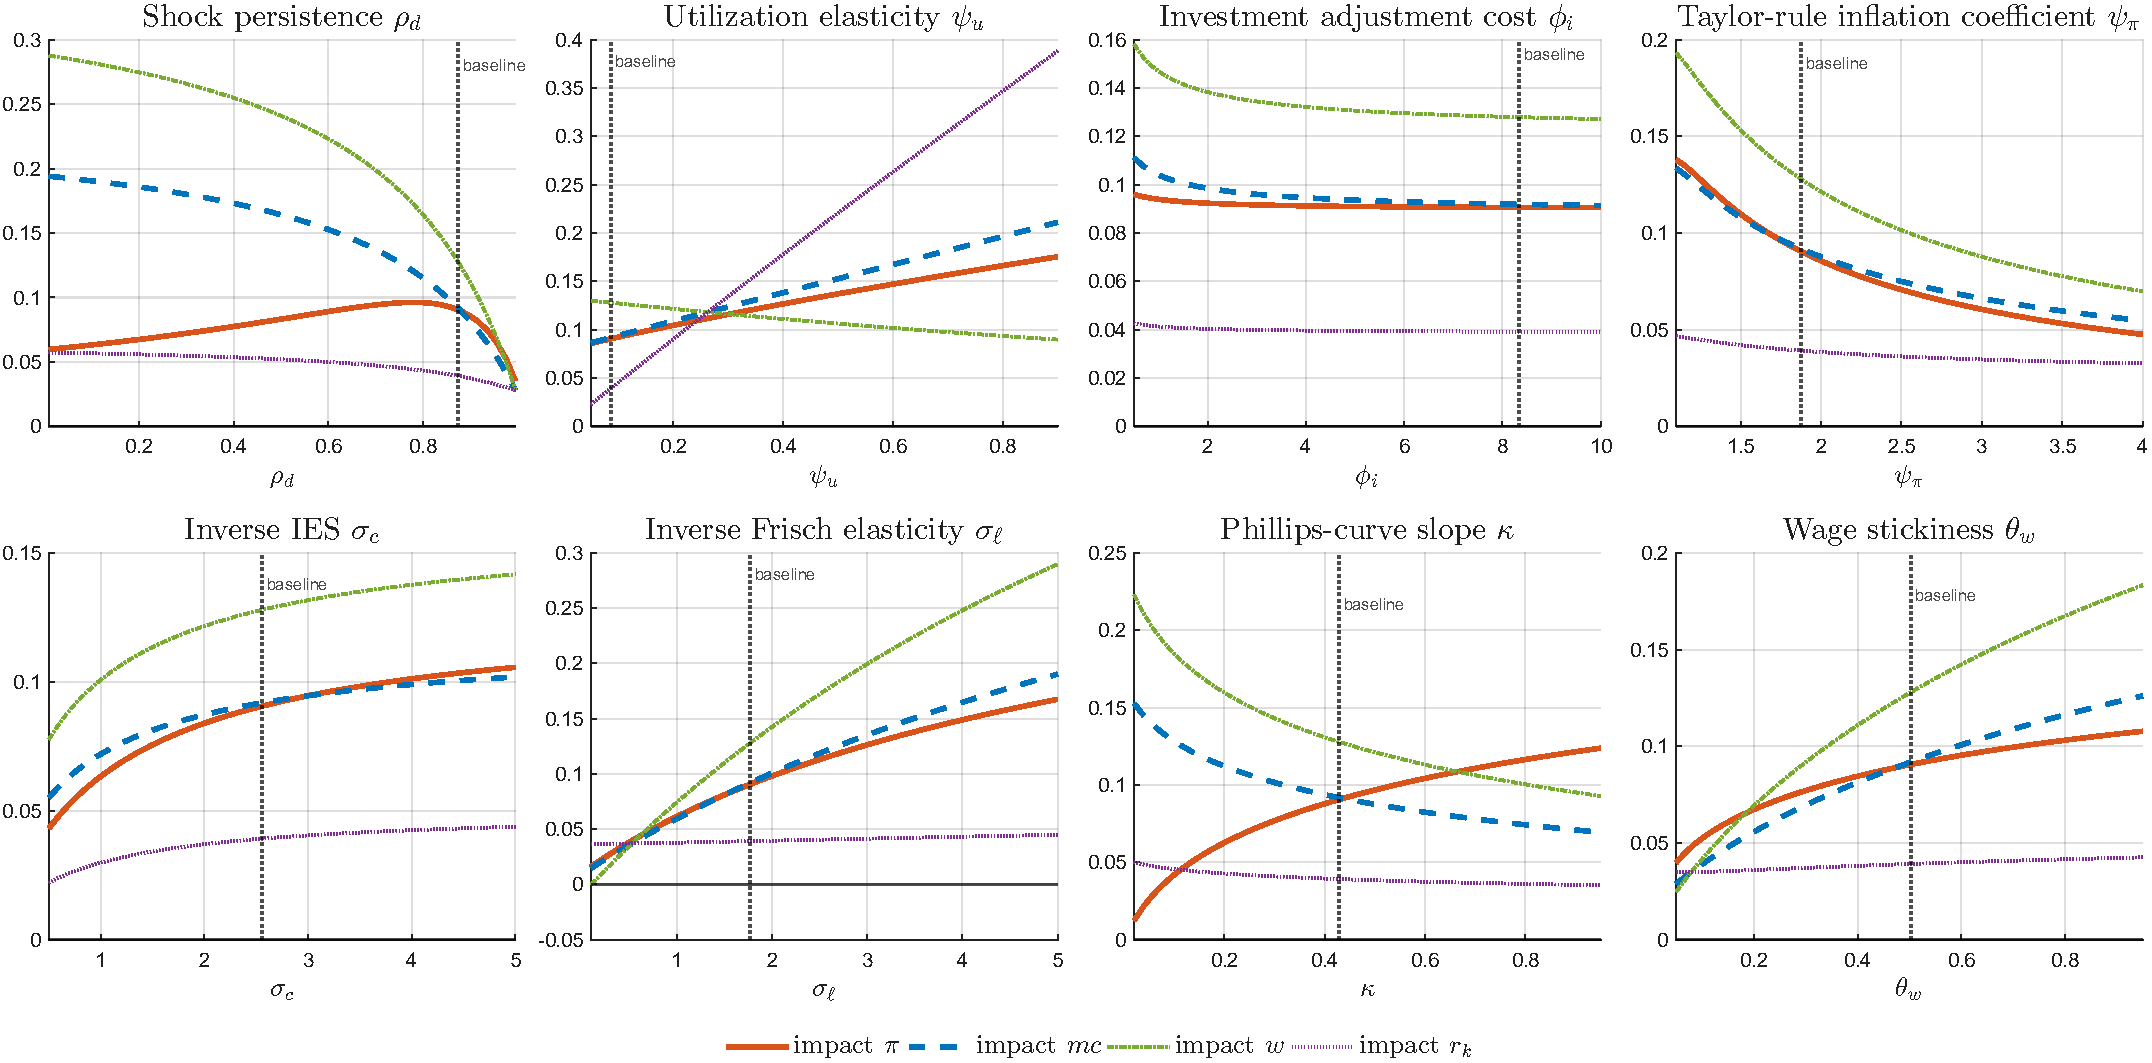
\includegraphics[width=\textwidth]{figures/inv_demand_sign_robustness.pdf}
    \caption{Robustness of the sign of the inflation response to an investment-demand shock. Each panel varies one parameter over a wide grid---the shock persistence \(\rho_d\), the capital-utilization elasticity \(\psi_u\), the investment adjustment cost \(\varphi_i\), and the Taylor-rule inflation coefficient \(\psi_\pi\)---holding all other parameters at the baseline posterior mean}
    \label{fig:inv_demand_sign_robustnes}
\end{figure}

\subsection{Consumption Impact}
\label{sec:results:con}
One of the attractions of the investment demand shock is its ability to generate comovements between consumption, investment and inflation, while the IST shock is usually unable to reproduce such a result. \cite{nireiOriginsPropagationAnimal} shows that the positive comovement shows up under certain calibrations, and one of the quests of this paper is to test whether the estimation supports such a result.

However, as shown in the IRF plot, Figure~\ref{fig:compare_irf}, the consumption impact is negative. Moreover, altering a single parameter value cannot reproduce a positive consumption impact either---such a result relies on certain parameter combinations. To figure out which parameter combination is needed, I align some model settings to \cite{nireiOriginsPropagationAnimal}, and simultaneously change three parameters that are important in theoretical proof---Phillips-curve slope \(\kappa_p\), the Taylor-rule inflation coefficient \(\psi_\pi\) and the wage-rigidity parameter \(\theta_w\). Result in Figure~\ref{fig:inv_demand_c1_kappa_psipi_heatmap} shows that, generally, if all three parameters are low enough, then consumption impact can be positive \footnote{Some may question about the indeterminate area in Figure~\ref{fig:inv_demand_c1_kappa_psipi_heatmap}, since the textbook new Keyasian model can be uniquely solven once $\psi_\pi > 1$. However, the problem becomes more complicated when capital and investment are added into the model, and \cite{sveen2005new} provides a detailed theoretical analysis about it.}. 

\begin{figure}
    \centering
    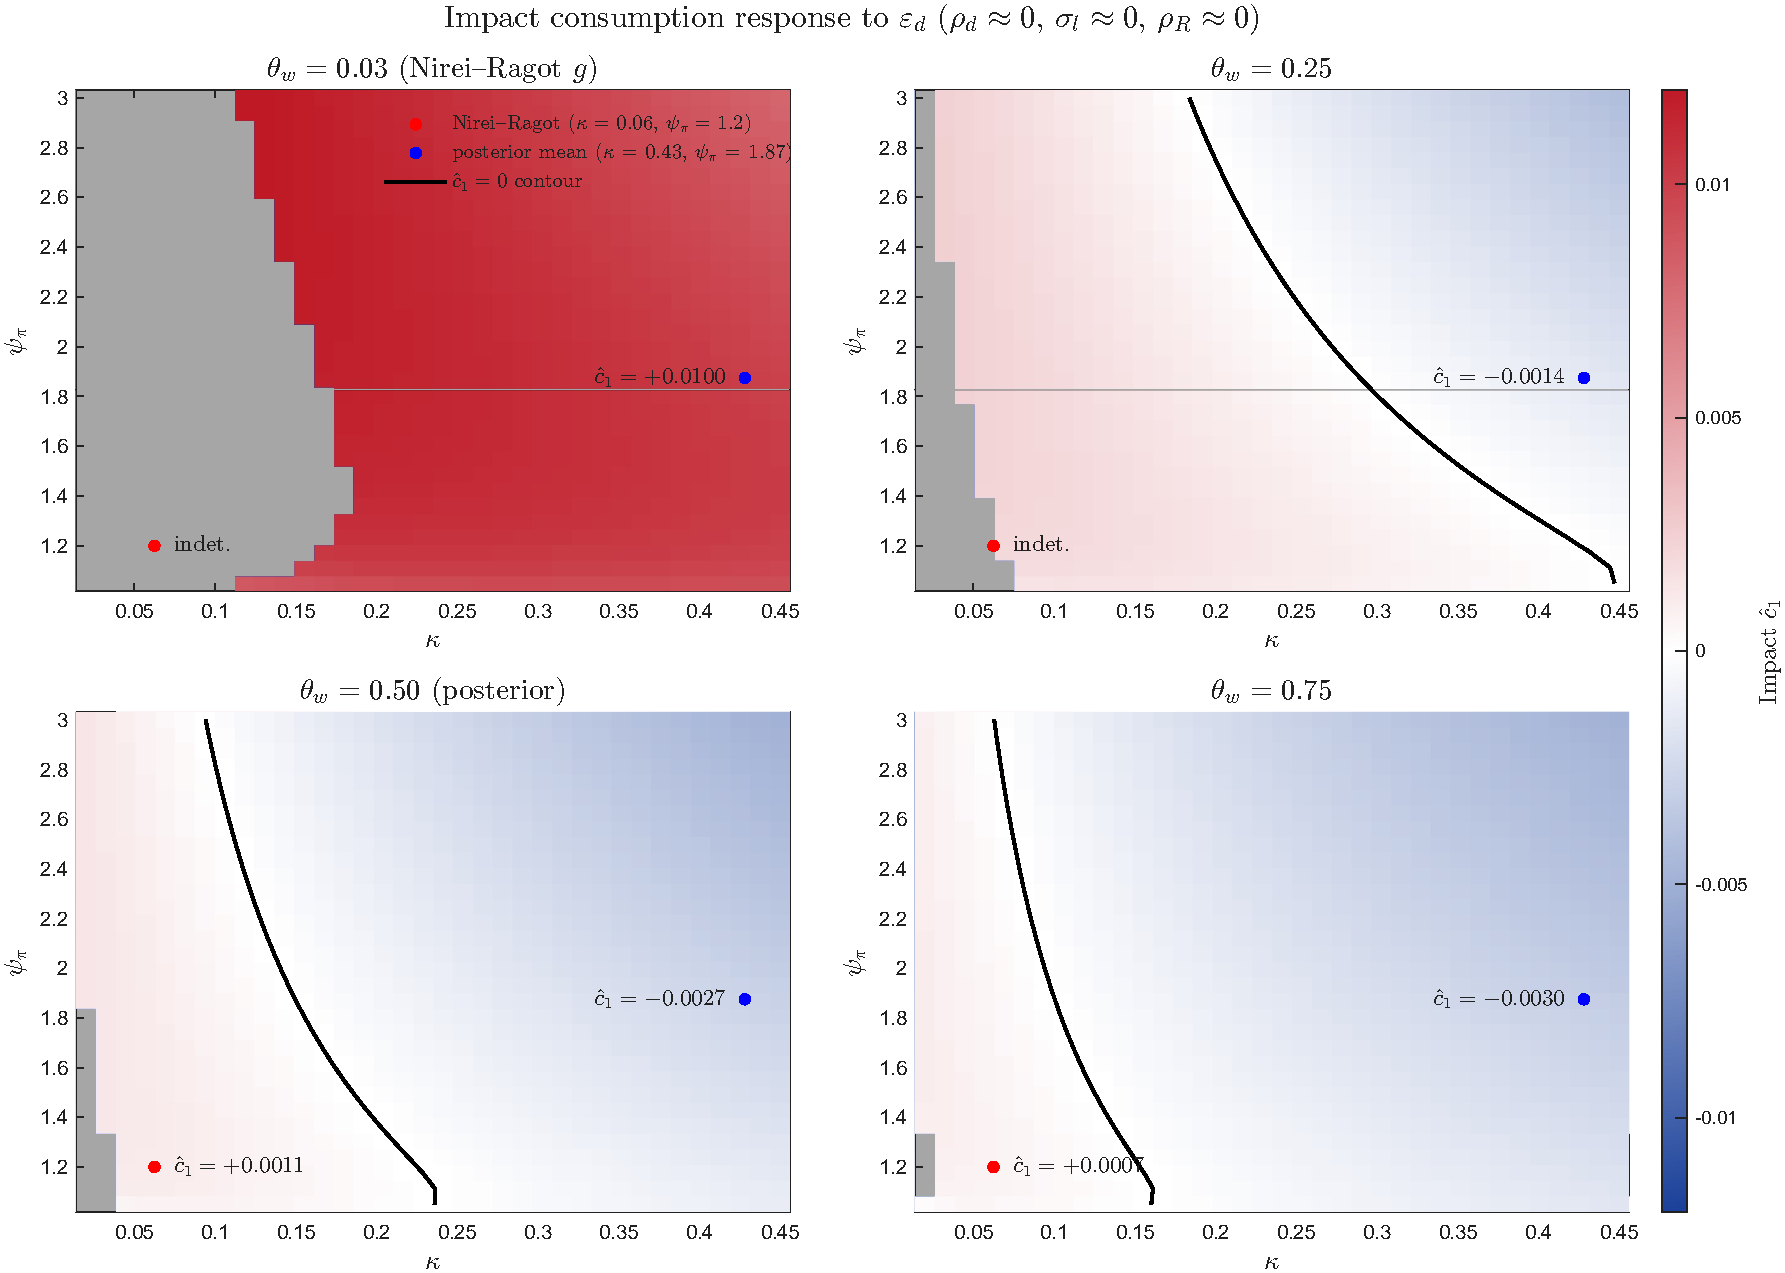
\includegraphics[width=\textwidth]{figures/inv_demand_c1_kappa_psipi_heatmap.pdf}
    \caption{Impact consumption response \(\hat c_1\) to a unit investment-demand shock as a function of the Phillips-curve slope \(\kappa_p\) and the Taylor-rule inflation coefficient \(\psi_\pi\) four values of the wage-rigidity parameter \(\theta_w\). The remaining parameters are held at the calibration in \cite{nireiOriginsPropagationAnimal}: an i.i.d. shock (\(\rho_d \approx 0\)), a non-inertial pure-inflation rule (\(\rho_R\approx 0\)), and near-linear labor disutility (\(\psi \approx 0\)). Gray cells are indeterminate configurations.}
    \label{fig:inv_demand_c1_kappa_psipi_heatmap}
\end{figure}

The result can be understand as follows. In short run, investment demand shock pushes up aggregate demand, but in long run accumulating more capital. Instead of investment, imagine that the capital increases directly. This simply makes households more wealthy, and thus they will consume more today. So, how to let the investment demand shock be analogous to direct capital increase? We can shut down the short-run effect by letting the economy to be more sticky---lower $\theta_w$ suppressing wage, lower $\kappa_p$ suppressing inflation, and lower $\psi_\pi$ suppressing nominal interest rate. They can then form a chain to suppress intertemporal substitution effect. If the wage increases only mildly, marginal cost will not increase much; if the Phillips curve is flat, inflation will not increase much; and if the Taylor rule is inactive to inflation, then the nominal interest rate will be stable; finally, since the real interest rate is stable, households will not shift today's consumption to tomorrow.

\subsection{Historical Decomposition}
\label{sec:results:hd}
To investigate the shock effects along the historical data, I show the historical decomposition in Figure~\ref{fig:hd:gov_data}, where the fluctuation of the fundamental macroeconomic data are decomposed into the fluctuation of structural shocks.

\begin{figure}
    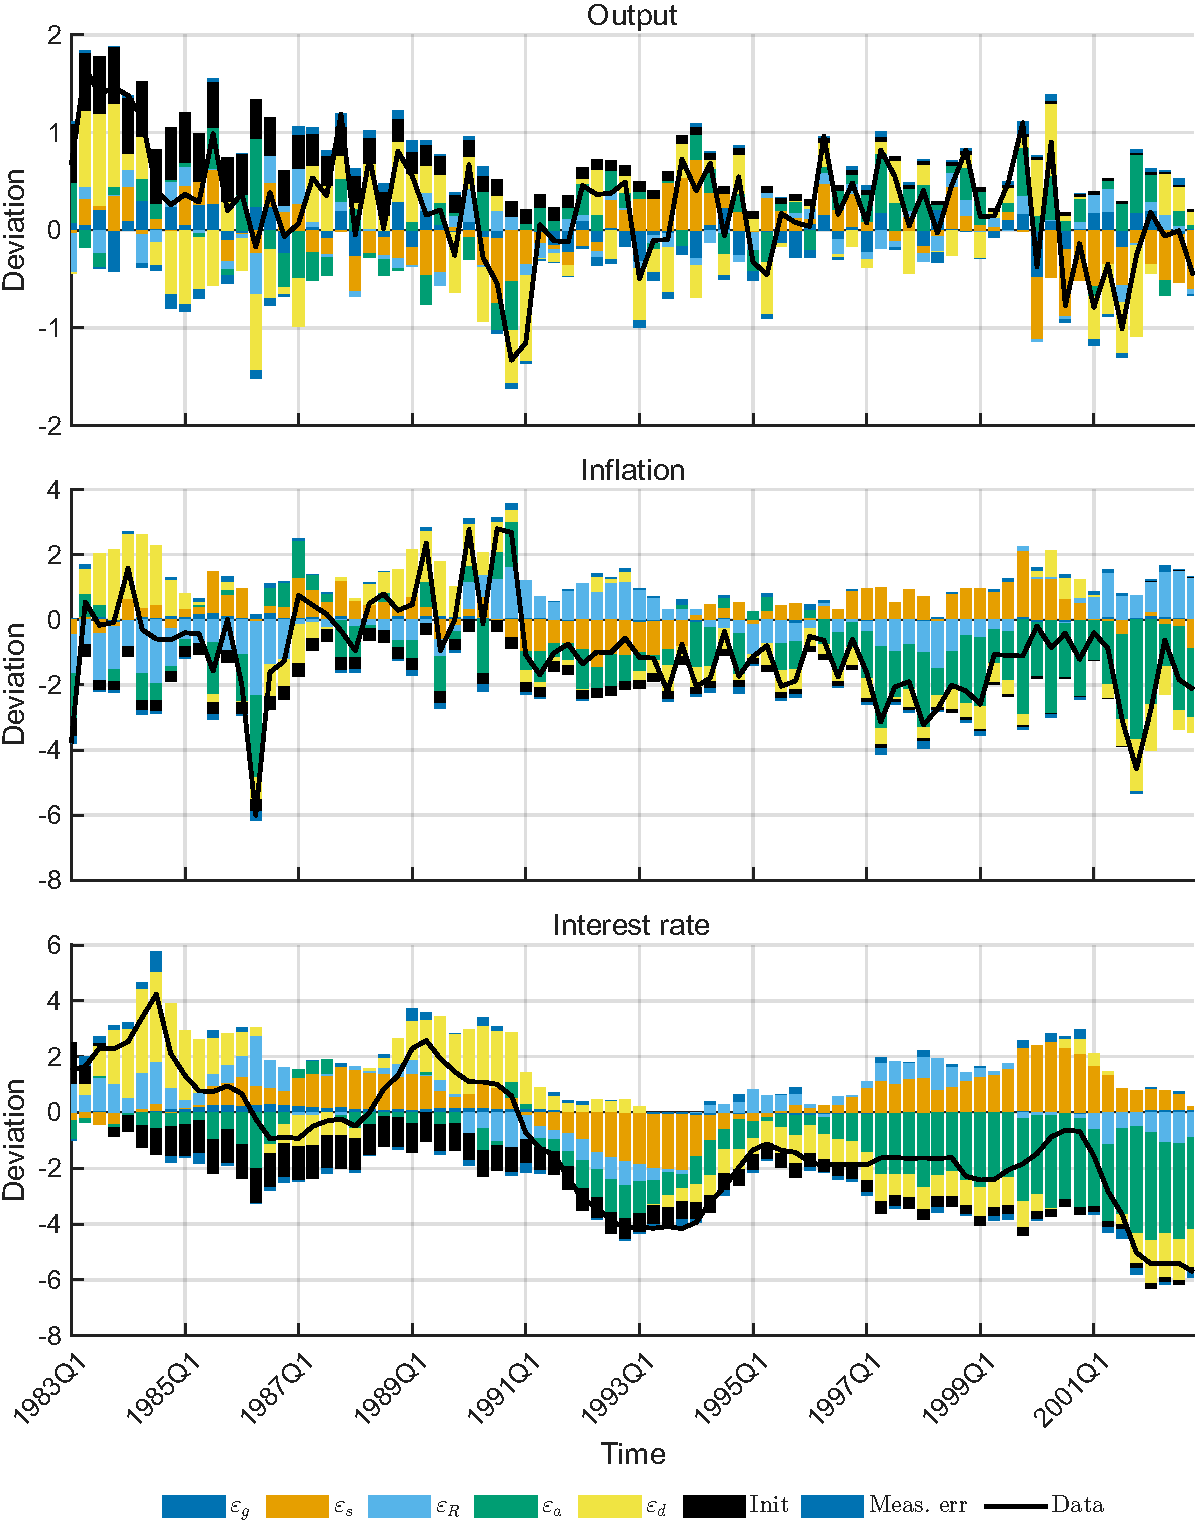
\includegraphics[width=0.9\textwidth]{figures/hd_gov_data.pdf}
    \caption{Historical decomposition (Kalman smoother) of demeaned output growth, inflation, and nominal interest rate into contributions from structural shocks (including initial conditions and measurement error) in the estimated baseline model.}
    \label{fig:hd:gov_data}
\end{figure}

Compared with the IST shock, the investment demand shock is shown to be more volatile in the HD of output, which often switches direction from quarter to quarter. Also, it behaves more procyclically, nearly moving in the same direction as output and inflation.

During the oil crisis in 1990-1991, both the IST shock and the investment demand shock show a very negative influence on output. After 1995, the aggregate productivity shock becomes the main driving force of inflation and the nominal interest rate. 